\documentclass[tikz,border=5pt]{standalone}
\usepackage{tikz}
\usetikzlibrary{positioning,fit,backgrounds,arrows.meta,calc}

\begin{document}
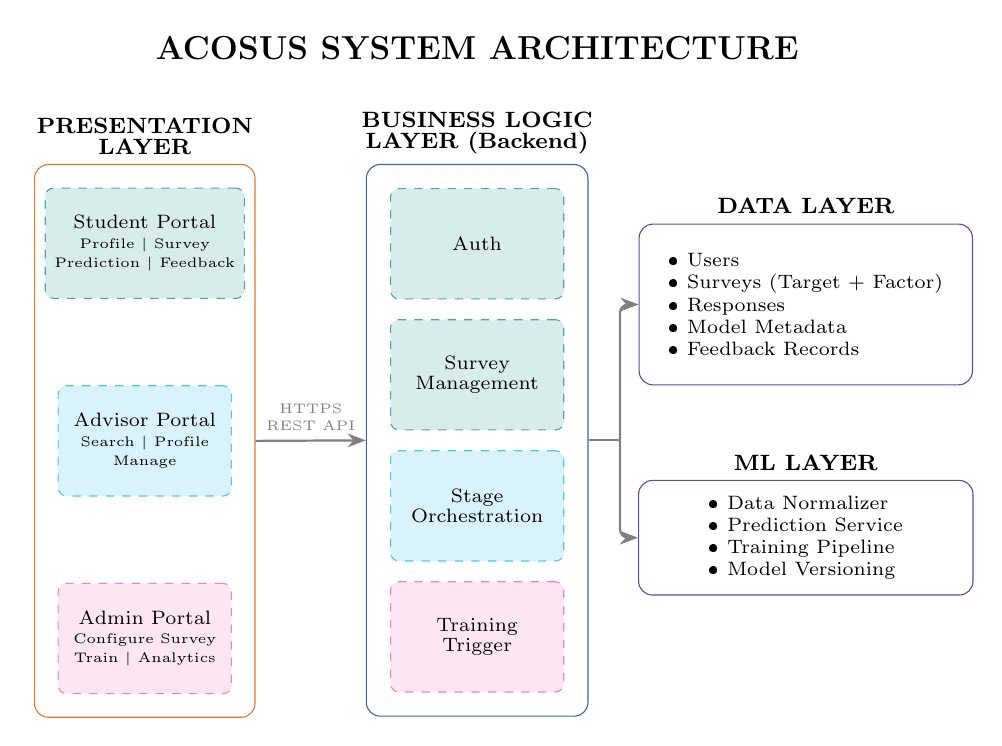
\begin{tikzpicture}[
    node distance=2.5mm,
    box/.style={draw, dashed, rounded corners=3pt, minimum width=22mm, minimum height=14mm, align=center, font=\scriptsize},
    layer/.style={draw, rounded corners=5pt, inner sep=3mm},
    student/.style={box, draw=teal!70, fill=teal!15},
    advisor/.style={box, draw=cyan!70, fill=cyan!15},
    admin/.style={box, draw=magenta!50, fill=magenta!10},
    lbl/.style={font=\footnotesize\bfseries, align=center},
    >=Stealth
]

\definecolor{orange}{RGB}{230,120,50}
\definecolor{dblue}{RGB}{60,100,180}
\definecolor{purple}{RGB}{100,70,170}

% Column 2: Business Logic Layer (reference)
\node[student] (auth) {Auth};
\node[student, below=of auth] (surv) {Survey\\[-1pt]Management};
\node[advisor, below=of surv] (stage) {Stage\\[-1pt]Orchestration};
\node[admin, below=of stage] (train) {Training\\[-1pt]Trigger};

\begin{scope}[on background layer]
\node[layer, draw=dblue, fit=(auth)(surv)(stage)(train), label={[lbl]above:BUSINESS LOGIC\\[-2pt]LAYER (Backend)}] (biz) {};
\end{scope}

% Column 1: Presentation Layer - create outer box first, then place inner boxes
\path let \p1=(biz.north), \p2=(biz.south), \p3=(biz.west) in
    node[layer, draw=orange, 
         minimum height={\y1-\y2}, 
         minimum width=28mm,
         anchor=north east,
         label={[lbl]above:PRESENTATION\\[-2pt]LAYER}] (pres) at ($(\x3,\y1)+(-14mm,0)$) {};

% Place boxes centered inside pres
\node[student, anchor=north] at ($(pres.north)+(0,-3mm)$) (sp) {Student Portal\\[-1pt]\tiny Profile \textbar{} Survey\\[-1pt]\tiny Prediction \textbar{} Feedback};
\node[advisor] at (pres.center) (ap) {Advisor Portal\\[-1pt]\tiny Search \textbar{} Profile\\[-1pt]\tiny Manage};
\node[admin, anchor=south] at ($(pres.south)+(0,3mm)$) (adm) {Admin Portal\\[-1pt]\tiny Configure Survey\\[-1pt]\tiny Train \textbar{} Analytics};

% Column 3: Data Layer (top) + ML Layer (bottom)
\node[right=12mm of auth, font=\scriptsize, align=left, anchor=north west] (dlist) {
    \textbullet\ Users\\
    \textbullet\ Surveys (Target + Factor)\\
    \textbullet\ Responses\\
    \textbullet\ Model Metadata\\
    \textbullet\ Feedback Records
};

\begin{scope}[on background layer]
\node[layer, draw=purple, fit=(dlist), inner sep=2.5mm, label={[lbl]above:DATA LAYER}] (data) {};
\end{scope}

% ML Layer - match Data Layer size
\path let \p1=(data.north), \p2=(data.south), \p3=(data.west), \p4=(data.east) in 
    node[below=12mm of data, layer, draw=purple, minimum height={\y1-\y2-6mm}, minimum width={\x4-\x3}, label={[lbl]above:ML LAYER}] (ml) {};

\node[font=\scriptsize, align=left] at (ml.center) {
    \textbullet\ Data Normalizer\\
    \textbullet\ Prediction Service\\
    \textbullet\ Training Pipeline\\
    \textbullet\ Model Versioning
};

% Title
\node[font=\large\bfseries, above=12mm of biz.north] (title) {ACOSUS SYSTEM ARCHITECTURE};

% Arrows
\draw[->, thick, gray] (pres.east) -- (biz.west) node[midway, above, font=\tiny, align=center] {HTTPS\\REST API};
\coordinate (split) at ($(biz.east)+(4mm,0)$);
\draw[thick, gray] (biz.east) -- (split);
\draw[->, thick, gray, rounded corners=3pt] (split) |- (data.west);
\draw[->, thick, gray, rounded corners=3pt] (split) |- (ml.west);

\end{tikzpicture}
\end{document}